%%% use 10pt options with the asme2ej format
\documentclass[10pt]{asme2ej}
\title{Re-implementation of the Adaptive Priority Queue With Elimination and Combining}
\usepackage{graphicx}
\usepackage{listings}

%%% first author
\author{Christopher L. Taliaferro
    \affiliation{
	Undergraduate\\
	Department of Computer Science\\
	University of Central Florida\\
    Email: guitartaliaferro@knights.ucf.edu
    }	
}

%%% second author
\author {Tiger Sachse
    \affiliation{
	Undergraduate\\
	Department of Computer Science\\
	University of Central Florida\\
    Email: tgsachse@knights.ucf.edu
    }	
}

%%% third author
\author{Ben Faria
    \affiliation{
	Undergraduate\\
	Department of Computer Science\\
	University of Central Florida\\
    Email: Benfaria96@knights.ucf.edu
    }	
}

%%% fourth author
\author{Harrison W. Black
    \affiliation{
	Undergraduate\\
	Department of Computer Science\\
	University of Central Florida\\
    Email: harrison.w.black@knights.ucf.edu
    }	
}

\begin{document}

\maketitle    

%%%%%%%%%%%%%%%%%%%%%%%%%%%%%%%%%%%%%%%%%%%%%%%%%%%%%%%%%%%%%%%%%%%%%%
\section{Introduction}

Priority queues are fundamental abstract data structures which can be implemented in a parallel fashion to assist in discrete event simulations and resource management \cite{latex}. Some of the current implementations of these parallel priority queues utilize heaps or skiplists to create the foundation, or main data structure to build these more abstract concurrent data structures. The skiplist implementation gives the ability to take advantage of the “potential for parallelism of the add method” \cite{latex}. 

%%%%%%%%%%%%%%%%%%%%%%%%%%%%%%%%%%%%%%%%%%%%%%%%%%%%%%%%%%%%%%%%%%%%%%
\section{Prior Implementations}
One skiplist-based implementation of the concurrent priority queue acts in a similar way to the “LazyList” and “LockFreeList” we have seen in the textbook, when a node is to be deleted it will be marked as such and then the thread will attempt to physically remove it, this implementation comes from Lotan and Shavit \cite{latex}. Another implementation of this concurrent priority queue comes from Hendler et al, this implementation introduced Flat Combining which batches together several operations and hand the batch to one thread to handle the execution of these operations \cite{latex}. This has also been taken and mixed in with a client server structure, where several client thread will create these operations to be handed off to a single server thread to then execute them. All these previous implementations have been steps in the right direction but they all have their flaws, the first implementation from Lotan and Shavit have the possibility of running into limited scalability when high thread counts are introduced due to contention on shared memory access. While the Flat Combining implementation reduces contention of the shared memory it introduces its own problem, which is the potential for the server thread to become a sequential bottleneck \cite{latex}.
%%%%%%%%%%%%%%%%%%%%%%%%%%%%%%%%%%%%%%%%%%%%%%%%%%%%%%%%%%%%%%%%%%%%%%
\section{Implementation with Elimination}
The implementations and their downsides lead to the implementation that is introduced and discussed in this paper, this being an implementation which uses a skiplist-based priority queue which employs an elimination algorithm. The skip list is used in this implementation because of its ability to provide both “operations-batching and disjoint-access parallelism.” \cite{latex}. As mentioned, part of this utilized the technique of batched operations from the Flat Combining implementation to improve the performance of the overall concurrent priority queue. As values are added into the priority queue they are subject to one of two paths, either the value is “small enough” to participate in elimination or it is too large and must be added into the skiplist normally. The second option mentioned is where the parallel portion of this data structure acts, high-values adds can be executed in parallel \cite{latex}. These two different paths that arise from adding to the skip list bring up the need for splitting the skip list into two different parts, being the sequential part handled by the server thread, and the parallel part \cite{latex}. The other side of this data structure comes from the remove min method which is where the batched operations comes into play, these “requests can be batched and executed by a server thread using the combining/delegation paradigm.” \cite{latex}. Designing the concurrent priority queue in this fashion allows for the reduction of contention and use of parallelism through elimination and high-valued adds \cite{latex}.
%%%%%%%%%%%%%%%%%%%%%%%%%%%%%%%%%%%%%%%%%%%%%%%%%%%%%%%%%%%%%%%%%%%%%%
\section{Interacting with Priority Queue}	
As mentioned, the design of this concurrent priority queue is based on an underlying skip list which is split into two parts, sequential and parallel, these two parts are both complete skip lists. The priority queue supports both the remove min method and the add method, the sequential part of the skip list will serve the remove min requests as well as the low-valued add requests which are more likely to be removed soon, while the parallel part will cater to the large-valued adds which are less likely to be removed in the near future \cite{latex}. Early the two paths that can be taken on an add request were touched on, but now they will be broken down further. When a priority queue add request is made two things happen, first the value is determined to be either less than or greater than the last value in the sequential list and from there it is passed on to its next step based on the condition it meets. If it is less than the last value the priority queue will attempt a remove min request using the elimination array which will be discussed further soon, otherwise if it is greater than the last value it will be sent to be added to the parallel list, which in turn means it will be added in parallel with any other values that met this same condition. As mentioned the add request of small values will in turn cause the thread to attempt to execute a remove min request that may exist in the elimination array. If there is no such request in the array, then the add request itself gets added to the elimination array. It will then wait in the elimination array until it either eliminates or times out, the server thread will sequentially execute any operations that fail to eliminate \cite{latex}.
%%%%%%%%%%%%%%%%%%%%%%%%%%%%%%%%%%%%%%%%%%%%%%%%%%%%%%%%%%%%%%%%%%%%%%
\section{Underlying Skiplist}
The sequential part of the skiplist uses a move head method to bring in elements form the parallel part when it becomes empty, it can also use a chop head method to relink the sequential and parallel portions in the case that there haven’t been remove min requests for some time \cite{latex}. These methods allow for the underlying skiplist to adjust based on the current state of the priority queue, either bringing in more elements from the parallel portion or linking with the parallel portion to perform more efficient parallel add requests. Anytime these move head and chop head methods are called the currSeq and lastSeq pointers are adjusted to represent the start and end to the new sequential part of the list thus allowing for the priority queue add and remove min requests to react to those changes. The parallel part of the list uses a “Single-Writer Multi-Readers lock” to ensure that and priority queue add requests are not operating on buckets that are being moved to the sequential part by the move head method or interferes with the chop head method \cite{latex}. A skip list find method is used to determine whether any head operations have been executed and if the find method comes back clean a lock \cite{lock} is held to avoid any head operations that take place after the clean find. This lock will then be released once a CAS fails while inserting a new value.
%%%%%%%%%%%%%%%%%%%%%%%%%%%%%%%%%%%%%%%%%%%%%%%%%%%%%%%%%%%%%%%%%%%%%%
\section{Elimination}
Now, with a better understanding of the structure and functionality if the underlying skiplist and its parts, the next major aspect of this concurrent priority queue is its elimination algorithm. In this priority queue, a remove min request can always be eliminated but if an add request finds its way into the elimination array it can only be eliminated if its value is less than or equal to the lowest value of the sequential portion of the list. The algorithm works by using an elimination array in which elements are added to the array and a remove min request searches through the “array until it finds a request to eliminate with or it finds an empty slot in the array” \cite{latex}. Once it finds one of these two things it will execute a CAS to get the value it needs to return, or it will fall through to the sequential part of the list and perform a remove and return that value. There are cases where an add request can never be eliminated if its value never goes below the lowest value in the priority queue. This is where the sequential server thread comes into play, it collects add and remove requests that fail to eliminate and executes them sequentially on the skiplist \cite{latex}. This functionality is key to the reduced contention of this concurrent priority queue.

%%%%%%%%%%%%%%%%%%%%%%%%%%%%%%%%%%%%%%%%%%%%%%%%%%%%%%%%%%%%%%%%%%%%%%
\section{Linearizability}

In this section we shall discuss the linearizability of our proposed method

%%%%%%%%%%%%%%%%%%%%%%%%%%%%%%%%%%%%%%%%%%%%%%%%%%%%%%%%%%%%%%%%%%%%%%
\subsection{Skiplist}

When implementing the Skiplist version of the priority queue, linearization occurs when an element is added to the parallel section of the skiplist, with addParallel(T). When this element is added, compare and swap \cite{cas} is invoked and the bucket for key T has its counter incremented, evoking linearization. If a thread inserts a new minimum value into our priority queue and the sequential part of the skiplist is empty, the thread then performs the required action of updating the queue’s minValue. If the sequential part of the list contains data, then the main thread synchronously updates minValue without linearization. Threads that succeed changing minValue linearize their operation at the point of the successful compare and swap. Some operations require the head of the list to be modified. The operations moveHead() and chopHead() execute while holding a lock. Linearization effectively occurs when the lock is released with lock.release().

%%%%%%%%%%%%%%%%%%%%%%%%%%%%%%%%%%%%%%%%%%%%%%%%%%%%%%%%%%%%%%%%%%%%%%
\subsection{Elimination}

Each thread, either adding or removing, that finds the inverse operation in the elimination array must verify that the exchanged value is smaller than minValue. If so, the thread can compare and swap the elimination slot, exchanging arguments with the waiting thread. It is possible that the priority queue minimum value is changed by a concurrent add(). In that case, the linearization point for the threads currently eliminating is when the value  observed is smaller than the priority queue minimum. The threads post their operation in the elimination array and wait for the main thread to process it. The main thread first marks the operation as in progress by compare and swapping ‘in progress´ into the slot. It then performs the sequential operation on the skiplist and writes the results back in the slot, releasing the waiting thread. The waiting thread gets the new value and returns it. The linearization point of this operation occurs when the sequential operation evokes on the skiplist.


%%%%%%%%%%%%%%%%%%%%%%%%%%%%%%%%%%%%%%%%%%%%%%%%%%%%%%%%%%%%%%%%%%%%%%
\section{Evaluation}

The author of the paper evaluated their results using the following benchmark. A thread randomly flips a coin with probability p to be an add() and 1 – p removeMin(). The tests began after inserting 2000 elements into the priority queue. Our priority queue algorithm is designed for high contention scenarios, in which elimination and combining thrive. Therefore, it can incur a penalty at lower thread counts. Although, our priority queue can fully take advantage of both elimination and parallel adds, so it maintains peak performance over other algorithms such as the flat combining skiplist, the flat combining pairing heap, the lock free skiplist, and the lazy skiplist at higher thread counts.

%%%%%%%%%%%%%%%%%%%%%%%%%%%%%%%%%%%%%%%%%%%%%%%%%%%%%%%%%%%%%%%%%%%%%%
\section{Hardware Transactions}

Regarding physical hardware transactions and the Adaptive Priority Queue, parallel threads are permitted speculatively execute critical sections. However, if two threads encounter a data conflict, one must roll back and re-execute its critical section. Results were evaluated using a Core i7-4770, running at 3.4GHz, with restricted transactional memory (RTM), and Hyperthreading enabled. Additionally, 8gb of RAM was shared and each core had 32KB of L1 cache\cite{latex}. 
\linebreak
\linebreak
\indent The sequential and parallel skiplists both use the Single-Write-Multi-Readers lock to synchronize. This causes complications with the priority queue as this lock adds a lot of overhead. Since the problem was approached by making all operations transactional, this lead to too many aborts occurring with this implementation. This was resolved by having the server increment a timestamp any time a head-moving operation like moveHead() or chopHead() starts or ends. Two operations are used to read a timestamp and then find the corresponding insertion. If a head-moving operation occurs after starting the transaction, the timestamp will change, causing the transaction to be aborted due to a timestamp conflict. For the timestamp to be valid the find() operation must record all predecessors and successors of a new bucket at each position i in preds[i] and succs[i]. If the bucket already exists, then the counter inside the transaction is incremented and the operation completes. The more threads running, the more increase in the number of transactions per successful operations. Additionally, the percentage of threads that need more than 10 tries to succeed also increases with the amount of threads running. After ten tries, threads stop attempting the transaction path and the server completes it for them. The amount of times this happens is at most 10 percent of the time but is generally less than 2 percent.

%%%%%%%%%%%%%%%%%%%%%%%%%%%%%%%%%%%%%%%%%%%%%%%%%%%%%%%%%%%%%%%%%%%%%%
\section{Our Implementation}

\subsection{Heap Implementation}
We decided to use a heap for our implementation of the priority queue for two main reasons, the first being the simplicity of the heap compared to the skiplist as well as doing a comparison between the performance of the priority queue when using a heap versus when using a skiplist. 

The main differences between the heap and the skiplist when it comes to the implementation are that the heap no longer supports a sequential and parallel portion of the data structure, this heap is entirely sequential which means that adds and removes are costlier due to the fact that multiple threads are modifying this heap at the same time. This lack of two separate portions as compared to the skiplist does simplify the implementation greatly, there is no need to support the moveHead and chopHead methods as discussed in the paper, which handle cases when the parallel and sequential portions of the skiplist become empty. Other than that, the functionality is very similar in that the heap allows for removal of the minimum value at a very inexpensive cost to performance, inserting into the heap as well as a method to peek, or get without removing the minimum value in the heap.

The major downside to using the heap are its lower efficiency in parallel environments as compared to the skiplist. As discussed in the paper, skiplists allow for disjoint-access parallelism which is very useful when it comes to inserting high valued priorities into the data structure. Because our heap implementation does not support parallel insertions as the skiplist does all insertions are handled by inserting into the heap and doing a CAS to check the validity of the insertion, this in turn is much costlier in terms of performance. 

Using the heap has its upsides too, the efficiency of the removeMin method is one, and another is the lack of a need for locks. The skiplist implementation requires the use of locks when performing actions on the parallel portion of the data structure, because we no longer have these two separate portions of our underlying data structure this is no longer a concern all insertions and removals can be handles using CAS. 

\subsection{Retrieve 'removeMin' method - Linearization}
The removeMin method in our implementation of the priority queue has four linearization points. These points are when the element is successfully removed from the elimination array, or in the case that the removal fails, the method linearizes when the element that has been marked as remove has been added to the elimination array. The other linearization point in the remove method is when the CAS on the pQueue variable succeeds otherwise when it returns null.

\begin{lstlisting}[language=Java]
public E retrieve() throws EmptyQueueException {
    Heap<E> currentpQueue = pQueue.get();
    Heap<E> updatedpQueue;

    CopyOnWriteArrayList<Element<E>> copiedElimination = new 
        CopyOnWriteArrayList<Element<E>>(elimination);
    Element<E> retVal;

    for(Element<E> object: copiedElimination) {
        if (currentpQueue.getMin() == null || (object.priority < 
                currentpQueue.getMin().priority && object.status == INSERT)) {
            int idx = copiedElimination.indexOf(object);
            retVal = copiedElimination.get(idx);
            if (!elimination.remove(object))
            {
                Element<E> newElement = 
                    new Element<E>(retVal.value, REMOVE, retVal.priority);
                elimination.add(newElement);
            }
            return retVal.value;
        }
    }

    do {
        currentpQueue = pQueue.get();
        updatedpQueue = new Heap<E>(currentpQueue);

        retVal = updatedpQueue.removeMin();
    }while (!pQueue.compareAndSet(currentpQueue, updatedpQueue));
    
    if(retVal == null) return null;

    return retVal.value;     
}
\end{lstlisting}

\subsection{Insert method - Linearization}
The insert method in our implementation contains three linearization points. The first of these points occurs when an element with a lower priority than the current minimum gets added to the elimination array. The other two linearization points occur when the element is successfully added to the pQueue and the CAS succeeds, otherwise when the value gets added to the elimination array.

\begin{lstlisting}[language=Java]
public void insert(E element) {
    Heap<E> currentpQueue = pQueue.get();
    Heap<E> updatedpQueue = new Heap<E>(currentpQueue);

    Element<E> inserting = new Element<>(element, INSERT, priotity.nextInt());
    Element<E> minValue = updatedpQueue.getMin();

    if (minValue == null || inserting.priority < minValue.priority) {
        elimination.add(inserting);
    }
    else {
        updatedpQueue.insert(inserting);

        if (!pQueue.compareAndSet(currentpQueue, updatedpQueue))
        {
            elimination.add(inserting);
        }
    }
}
\end{lstlisting}

\subsection{Run method - Linearization}
The run method in our implementation is run by the single server thread and it contains two linearization points. The first of these points occurs when an element is successfully removed from the pQueue and thus removed from the elimination array. Similarly, the other linearization point occurs when the element is successfully added to the pQueue and the CAS succeeds and the element gets removed from the elimination array. 

\begin{lstlisting}[language=Java]
 public void run(){
    while (isRunning) {
        Heap<E> currentpQueue;
        Heap<E> updatedpQueue;
        CopyOnWriteArrayList<Element<E>> copiedElimination = new 
            CopyOnWriteArrayList<Element<E>>(elimination);
            
        for(Element<E> object: copiedElimination) {
            if (object.status == REMOVE)
            {
                do {
                    currentpQueue = pQueue.get();
                    updatedpQueue = new Heap<E>(currentpQueue);
                    updatedpQueue.removeMin();
                }while (!pQueue.compareAndSet(currentpQueue, updatedpQueue));
                elimination.remove(object);
            }
            else if (object.status == INSERT){
                currentpQueue = pQueue.get();
                updatedpQueue = new Heap<E>(currentpQueue);
                updatedpQueue.insert(object);

                if (pQueue.compareAndSet(currentpQueue, updatedpQueue))
                    elimination.remove(object);
            }
        }
    }
}
\end{lstlisting}

\subsection{Correctness}
This implementation of the priority queue is correct in that it adheres to the proper functionality of a priority queue with elimination and combining. In this case that one thread is performing an insert at the same time as another thread is performing a removal, if the insert successfully adds to elimination array the write will change the elimination array so as the removal iterates through the array it will see the insertion and eliminate with it if necessary. The insertion could also insert into the pQueue in which case it will try to CAS and as long as the removal has not change the pQueue while the insert has taken place it will succeed. Another case would be the server thread performing a removal or insertion while another thread is performing another action, this case will work out similar as it will use CAS to successfully remove or insert to the pQueue.

\subsection{Physical Hardware}
All runtime analysis was performed on a 2010 MacBook Pro. The MacBook Pro uses a Intel Core 2 Duo processor, running at 2.4 Ghz, without hyperthreading. It uses 8 Gbs of RAM shared between the two cores with each core having 32Kbs of L1 cache.

\subsection{Software Transactional Memory}
Our implementation of Software Transactional Memory uses the Java Deuce STM framework. Java Deuce is an open-source project that makes no direct changes to Java. It is a runtime environment that makes use of byte code manipulation to accomplish its task. Deuce comes with a simple API, requiring nothing more than placing an “@Atomic” above the function you wish to implement STM on. It is made this easy due to the fact Java Deuce is field based, which in turn gives it great scalability. Under the hood, Deuce supports two main mechanisms to handle Transaction flow. First, Deuce has a “TransactionException.” When thrown, the current context of a running transaction will be rolled back and a new transaction will retry the previous action. Second, Deuce has a “AbortTransactionException.” When thrown the current context of a running transaction will be rolled back and aborted. Unlike most concurrency strategies, which are implemented in hardware, STM is implemented in software. For STM a transaction occurs when a section of the code executes multiple reads and writes to the shared memory of the cores. All of these actions happen at the same time instance. STM essentially makes a list of things to do and then sends that list off to memory to have all those things done at once. If the transaction fails, it will continue to retry until the transaction is successful or aborted.

When examining the graphs, the number of threads running has a noticeable effect on runtimes. If less than four threads are used, using Deuce STM is almost always the worst choice. This is due to the fact that STM must maintain a log of memory transactions. The overhead of maintaining the log and the time spent committing transactions is so demanding it is not worth using STM without at least five threads running. Another large performance factor was the amount of pops that occur. Sice STM works by batching actions together and then sending it to memory, when a large amount of pops occur, STM is really sending a large amount of reads to the memory. Reads take a longer amount of time to occur than writes do. This is because a CPU can move forward as soon as the instruction to write is given. The CPU does not need the write to complete before continuing because writing has no effect on the next action. However for reads, the core must wait for the instruction to complete and the data to make its way back to the core before continuing. This issue then compounds with the fact that if the transaction fails it must roll back and retry the transaction. 

STM is at no point the best of the three implementations but it tends perform better than the Synchronized Priority Queue so long as the push to pop ratio is greater than 3:1. 
At 2:1, STM and the SPQ are tied once STM gets past its four thread hump. Around a 3:2 push to pop ratio, STM becomes the worst choice of the three.

\subsection{Performance}
When our 3 implementations are executed with significantly more pops than pushes per thread across
32 threads, the transactional memory is out-performed by the simple synchronous implementation, and
the elimination-and-combining (EC) implementation performs better than both. The poor performance
caused by the transactional memory implementation is likely due to the high overhead of using transactions on a data structure that is usually empty (because the data structure experiences more pops than pushes). Also, the great performance of the EC implementation is likely explained by a decreased need for the elimination array. If most operations on the EC implementation are pops, the elimination array is mostly empty, as is the rest of the data structure, and so the array is not visited as often.

\begin{figure}[htp]
\centering
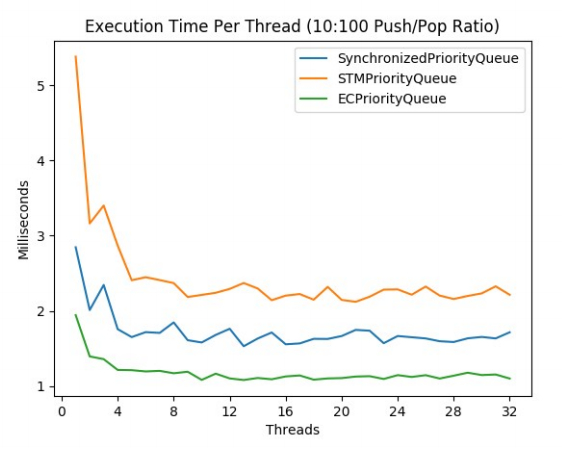
\includegraphics[width=6cm]{1.jpg}
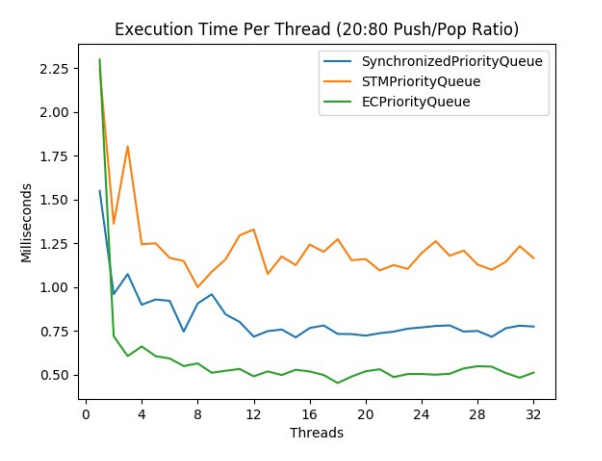
\includegraphics[width=6.5cm]{2.jpg}
\end{figure}

When our 3 implementations are executed with significantly more pushes than pops, the performance
of the transactional memory and synchronous implementations flip. In this situation, the performance
hit of utilizing transactional memory is less important than the extreme contention on the synchronous implementation caused by Java’s “synchronous” keyword. The execution time of the EC
implementation is still quite low, and we suspect this is for the same reason as mentioned previously: the elimination array is not needed as much when the ratio of pushes to pops on the EC implementation is uneven.

\begin{figure}[htp]
\centering
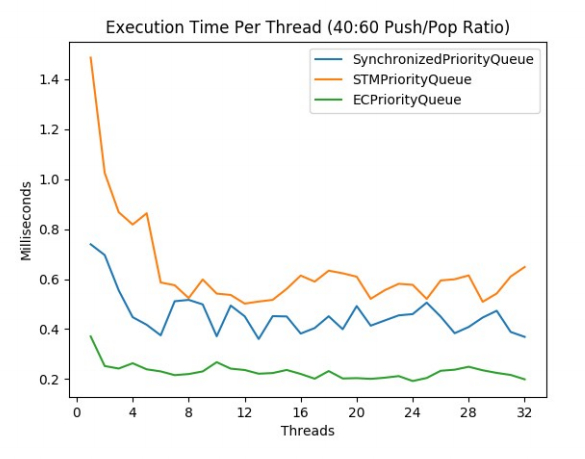
\includegraphics[width=5.9cm]{3.jpg}
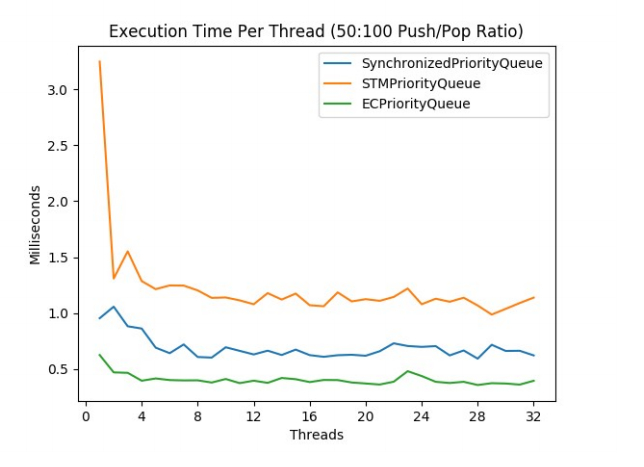
\includegraphics[width=6.5cm]{4.jpg}
\end{figure}

\begin{figure}[htp]
\centering
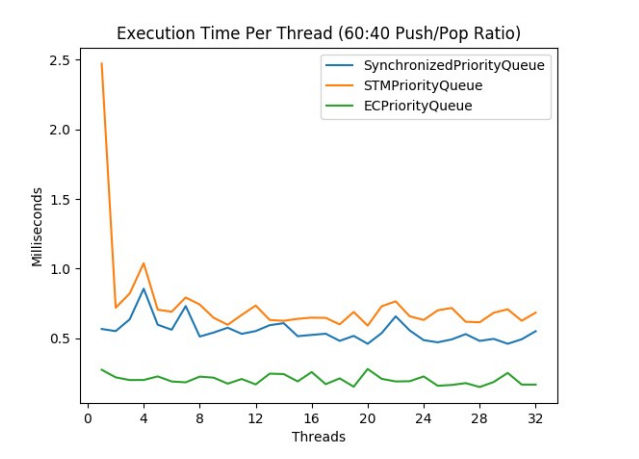
\includegraphics[width=6cm]{5.jpg}
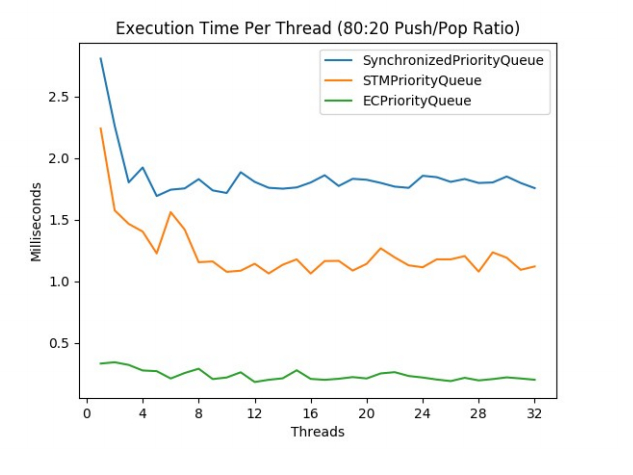
\includegraphics[width=6cm]{6.jpg}
\end{figure}

The final graph, which shows an even push to pop ratio executed on our implementations, is the most
interesting graph of the 9. This graph shows that the EC implementation significantly under-performs
compared to the STM and synchronized implementations. We suspect this is due to high contention on
the elimination array in the EC implementation. With an even ratio of operations directed at our data
structure, the EC implementation has to frequently access the elimination array. This access is
expensive and results in a visible slowdown.

\begin{figure}[htp]
\centering
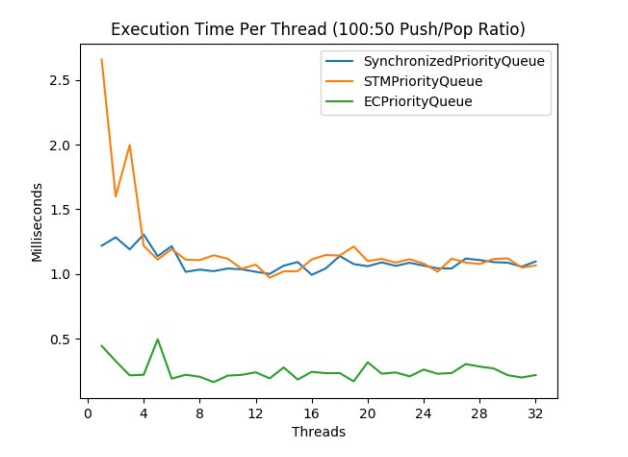
\includegraphics[width=6cm]{7.jpg}
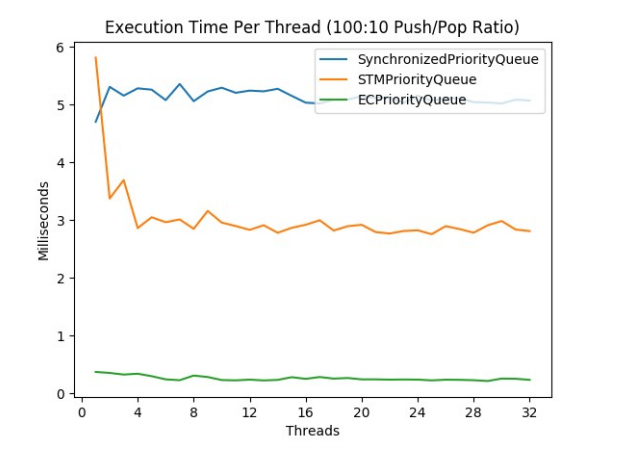
\includegraphics[width=6cm]{8.jpg}
\end{figure}

Our conclusion given this data is that the elimination-and-combining priority queue is the best choice for unbalanced workloads (an uneven ratio of pushes to pops). If one suspects that his data structure will experience an even ratio, he might choose to stick with simplicity and use a synchronized queue instead.

\begin{figure}[htp]
\centering
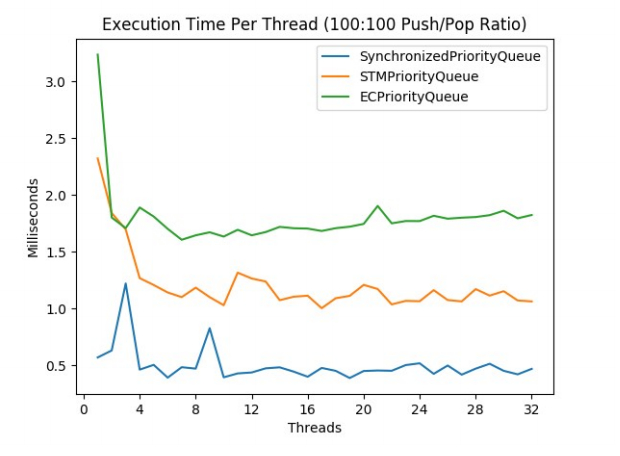
\includegraphics[width=6cm]{9.jpg}
\end{figure}

%%%%%%%%%%%%%%%%%%%%%%%%%%%%%%%%%%%%%%%%%%%%%%%%%%%%%%%%%%%%%%%%%%%%%%
% Here's where you specify the bibliography style file.
% The full file name for the bibliography style file 
% used for an ASME paper is asmems4.bst.
\bibliographystyle{asmems4}

% Here's where you specify the bibliography database file.
% The full file name of the bibliography database for this
% article is asme2e.bib. The name for your database is up
% to you.
\bibliography{asme2e}
%%%%%%%%%%%%%%%%%%%%%%%%%%%%%%%%%%%%%%%%%%%%%%%%%%%%%%%%%%%%%%%%%%%%%%

\end{document}
